\documentclass[a4paper,11pt]{article}

\usepackage{préambule}
\usetikzlibrary{arrows,positioning,arrows.meta}

\renewcommand{\baselinestretch}{1.7}

\newcommand{\myarrow}{-{Latex[length=3mm, width=2mm]}}

\makeatletter
\renewcommand{\maketitle}{%
    \topskip1em
	\@author \hfill \@date \\

	\begin{center}
		\begin{huge}
			\@title \\[1em]
		\end{huge}
	\end{center}
}
\makeatother

\title{Contrôle : nombres relatifs}
\date{7 janvier}
\author{Prénom : {\color{red} CORRECTION}}

\begin{document}

\maketitle

\begin{question}[(4 points)]
	Donner l'abscisse des points A, B, C et D : \vspace{1em}

	\begin{center}
		\begin{tikzpicture}
			\draw[\myarrow] (-5.5,0) -- (5.5,0);
			\foreach \x in {-5,...,5} {
					\draw (\x,0) -- (\x,-0.2);
				}
			\node[below] at (0,-0.2) {0};
			\node[below] at (1,-0.2) {1};

			\coordinate (A) at (2,0);
			\coordinate (B) at (-2,0);
			\coordinate (C) at (-3.5,0);
			\coordinate (D) at (0.5,0);

			\foreach \p in {A,B,C,D} {
					\node at (\p) {×};
					\node[above] at (\p) {\p};
				}
		\end{tikzpicture}
	\end{center}

	{\color{red}\begin{tabular}{ll}
		A a pour abscisse 2.    & B a pour abscisse -2.  \\
		C a pour abscisse -3,5. & D a pour abscisse 0,5.
	\end{tabular}} \vspace{1em}

	Donner l'abscisse des points E, F, G et H : \vspace{1em}

	\begin{center}
		\begin{tikzpicture}[scale=6]
			\draw[\myarrow] (-1.1,0) -- (1.1,0);
			\foreach \x in {-5,...,5} {
					\draw (\x / 5,0) -- (\x / 5,-0.04);
				}
			\node[below] at (-0.4,-0.04) {-0,4};
			\node[below] at (-0.6,-0.04) {-0,6};

			\coordinate (E) at (0.7,0);
			\coordinate (F) at (-0.2,0);
			\coordinate (G) at (-0.4,0);
			\coordinate (H) at (-1,0);

			\foreach \p in {E,F,G,H} {
					\node at (\p) {×};
					\node[above] at (\p) {\p};
				}
		\end{tikzpicture}
	\end{center}

	{\color{red}\begin{tabular}{ll}
		E a pour abscisse 0,7.  & F a pour abscisse -0,2. \\
		G a pour abscisse -0,4. & H a pour abscisse -1.
	\end{tabular}}
\end{question}

\begin{question}[(3 points)]
	Complète par $<$ ou $>$ :

	\begin{multicols}{3}
		\begin{enumerate}[a)]
			\item 5 {\color{red} >} 3
			\item -5 {\color{red} <} -3
			\item -8,51 {\color{red} <} -8,5
			\item -7,12 {\color{red} <} 0,8
			\item 3,14 {\color{red} >} 2,718
			\item -0,99 {\color{red} <} -0,909
		\end{enumerate}
	\end{multicols}
\end{question}

\begin{question}[(2 points)]
	\begin{enumerate}[1)]
		\item Range les nombres suivants dans l'ordre croissant :

		      5 ; 2,7 ; -2,6 ; -0,1 ; 7,1 ; -8,3

		      {\color{red} -8,3 < -2,6 < -0,1 < 2,7 < 5 < 7,1}
		\item Range les nombres suivants dans l'ordre décroissant :

		      -10,6 ; 14 ; -8,31 ; -3,8 ; 4,2 ; -8,3

		      {\color{red} 14 > 4,2 > -3,8 > -8,3 > -8,31 > -10,6}
	\end{enumerate}
\end{question}

\begin{question}[(4 points)]\

	\begin{minipage}{0.45\textwidth}
		Donne les coordonnées des points A, B, C, D, E, F, G et H.

			{\color{red}\begin{tabular}{ll}
					A(2 ; 3) \hspace{3em} & B(-3 ; 0) \\
					C(0 ; 2)              & D(3 ; 2)  \\
					E(4 ; 0)              & F(3 ; -2) \\
					G(-5 ; -3)            & H(-2 ; 3)
				\end{tabular}}
	\end{minipage} \hspace{1em}
	\begin{minipage}{0.45\textwidth}
		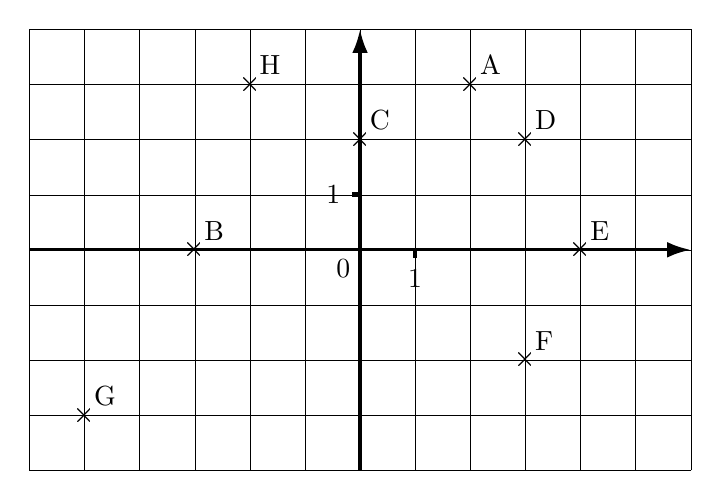
\begin{tikzpicture}[scale=0.7]
			\draw[ultra thin] (-6,-4) grid (6,4);
			\draw[very thick,\myarrow] (-6,0) -- (6,0);
			\draw[very thick,\myarrow] (0,-4) -- (0,4);
			\draw[ultra thick] (1,0) -- (1,-0.15) node[below] {1};
			\draw[ultra thick] (0,1) -- (-0.15,1) node[left] {1};
			\node[below left] at (0,0) {0};

			\coordinate (A) at (2,3);
			\coordinate (B) at (-3,0);
			\coordinate (C) at (0,2);
			\coordinate (D) at (3,2);
			\coordinate (E) at (4,0);
			\coordinate (F) at (3,-2);
			\coordinate (G) at (-5,-3);
			\coordinate (H) at (-2,3);

			\foreach \p in {A,B,C,D,E,F,G,H} {
					\node at (\p) {×};
					\node[above right] at (\p) {\p};
				}
		\end{tikzpicture}
	\end{minipage}
\end{question}

\newpage

\begin{question}[(7 points)]\

	Trace un repère dans l'espace ci-dessous.

	\begin{center}
		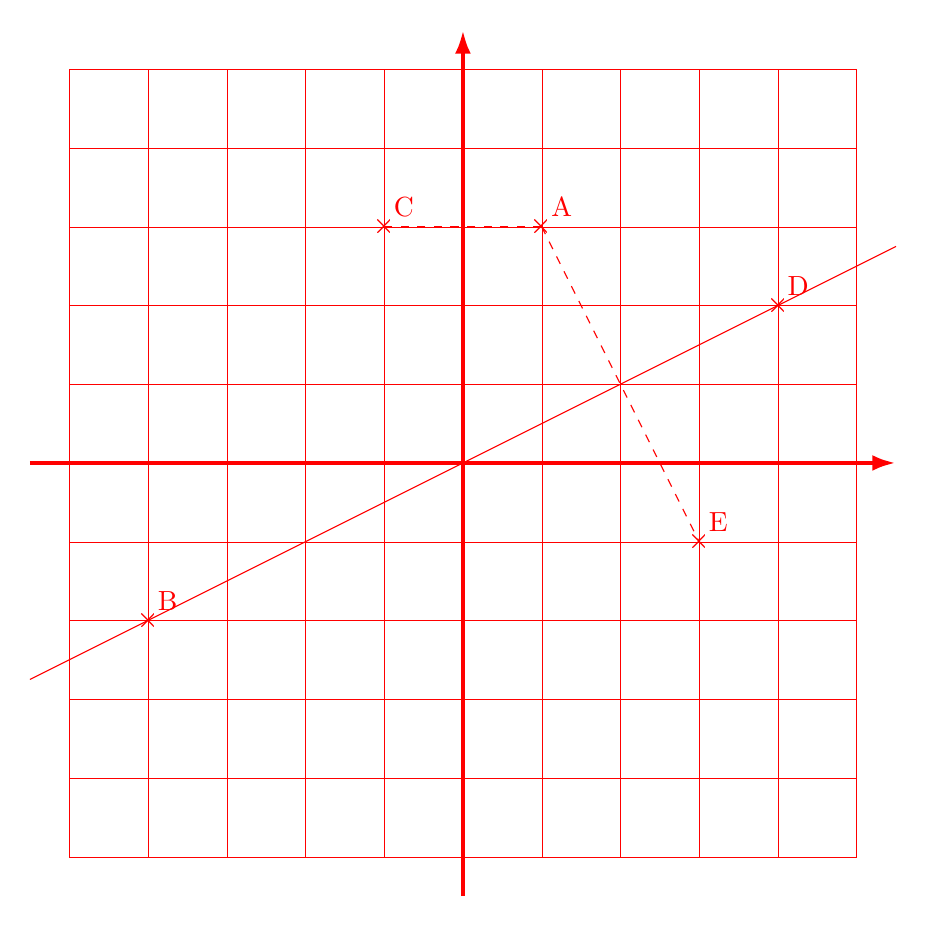
\begin{tikzpicture}
			\draw[red,ultra thin] (-5,-5) grid (5,5);
			\draw[red,ultra thick,\myarrow] (-5.5,0) -- (5.5,0);
			\draw[red,ultra thick,\myarrow] (0,-5.5) -- (0,5.5);

			\coordinate (A) at (1,3);
			\coordinate (B) at (-4,-2);
			\coordinate (C) at (-1,3);
			\coordinate (D) at (4,2);
			\coordinate (E) at (3,-1);

			\draw[red] (-5.5,-2.75) -- (5.5,2.75);
			\draw[red,dashed] (A) -- (E);
			\draw[red,dashed] (A) -- (C);

			\foreach \p in {A,B,C,D,E} {
					\node[red] at (\p) {×};
					\node[red,above right] at (\p) {\p};
				}
		\end{tikzpicture}
	\end{center}

	\begin{enumerate}[1)]
		\item Place le point A de coordonnées (1 ; 3).
		\item Place le point B de coordonnées (-4 ; -2).
		\item Place le point C symétrique de A par rapport à \textbf{l'axe des ordonnées}. Quelles sont ses coordonnées ? {\color{red} (-1 ;3)}
		\item Place le point D symétrique de B par rapport à \textbf{l'origine}. Quelles sont ses coordonnées ? {\color{red} (4 ;2)}
		\item Trace la droite (BD).
		\item Place le point E symétrique de A par rapport à \textbf{la droite (BD)}.  Quelles sont ses coordonnées ? {\color{red} (3 ; -1)}
	\end{enumerate}
\end{question}

\end{document}